\documentclass{beamer}

\usepackage[english]{babel}
\usepackage[utf8]{inputenc}

\usepackage{amsmath}[]
\usepackage{graphicx}
\usepackage{braket}
\usepackage{multimedia}
\usepackage[squaren]{SIunits}

\newcommand{\Bd}{$B_d^0$}
\newcommand{\Bdbar}{$\overline{B_d^0}$}
\newcommand{\SJPsi}{S_{J/\Psi K_s^0}}


\usetheme{Luebeck}
\usecolortheme{default}
\usefonttheme{default}
\useinnertheme{default}
\useoutertheme{default}
    \defbeamertemplate{footline}{author and page number}{%
      \usebeamercolor[fg]{page number in head/foot}%
      \usebeamerfont{page number in head/foot}%
      \hspace{1em}\insertshortauthor\hfill\insertshorttitle\hfill%
      \insertpagenumber\,/\,\insertpresentationendpage\kern1em\vskip2pt%
    }
\setbeamertemplate{footline}[author and page number]{}
\setbeamertemplate{navigation symbols}{}    



\title[Measurement of $\sin(2\beta)$]{Measurement of $\sin(2\beta)$ in the decay $B_d^0 \longrightarrow J/\Psi K_s^0$}
\subtitle[]{}
\author[Johannes Mayer, Patrick Fahner]{Johannes Mayer, Patrick Fahner}
\institute[]{LHCb, Physikalisches Institut \\ Heidelberg University}
\date[27.05.13]{27. Mai 2013}
\subject{}
\keywords{}

\begin{document}
\setlength\abovedisplayskip{0pt}
	\begin{frame}[plain]
	\titlepage
	\end{frame}
	
	\begin{frame}{Decay $B_d^0 \longrightarrow J/\Psi K_s^0$}
	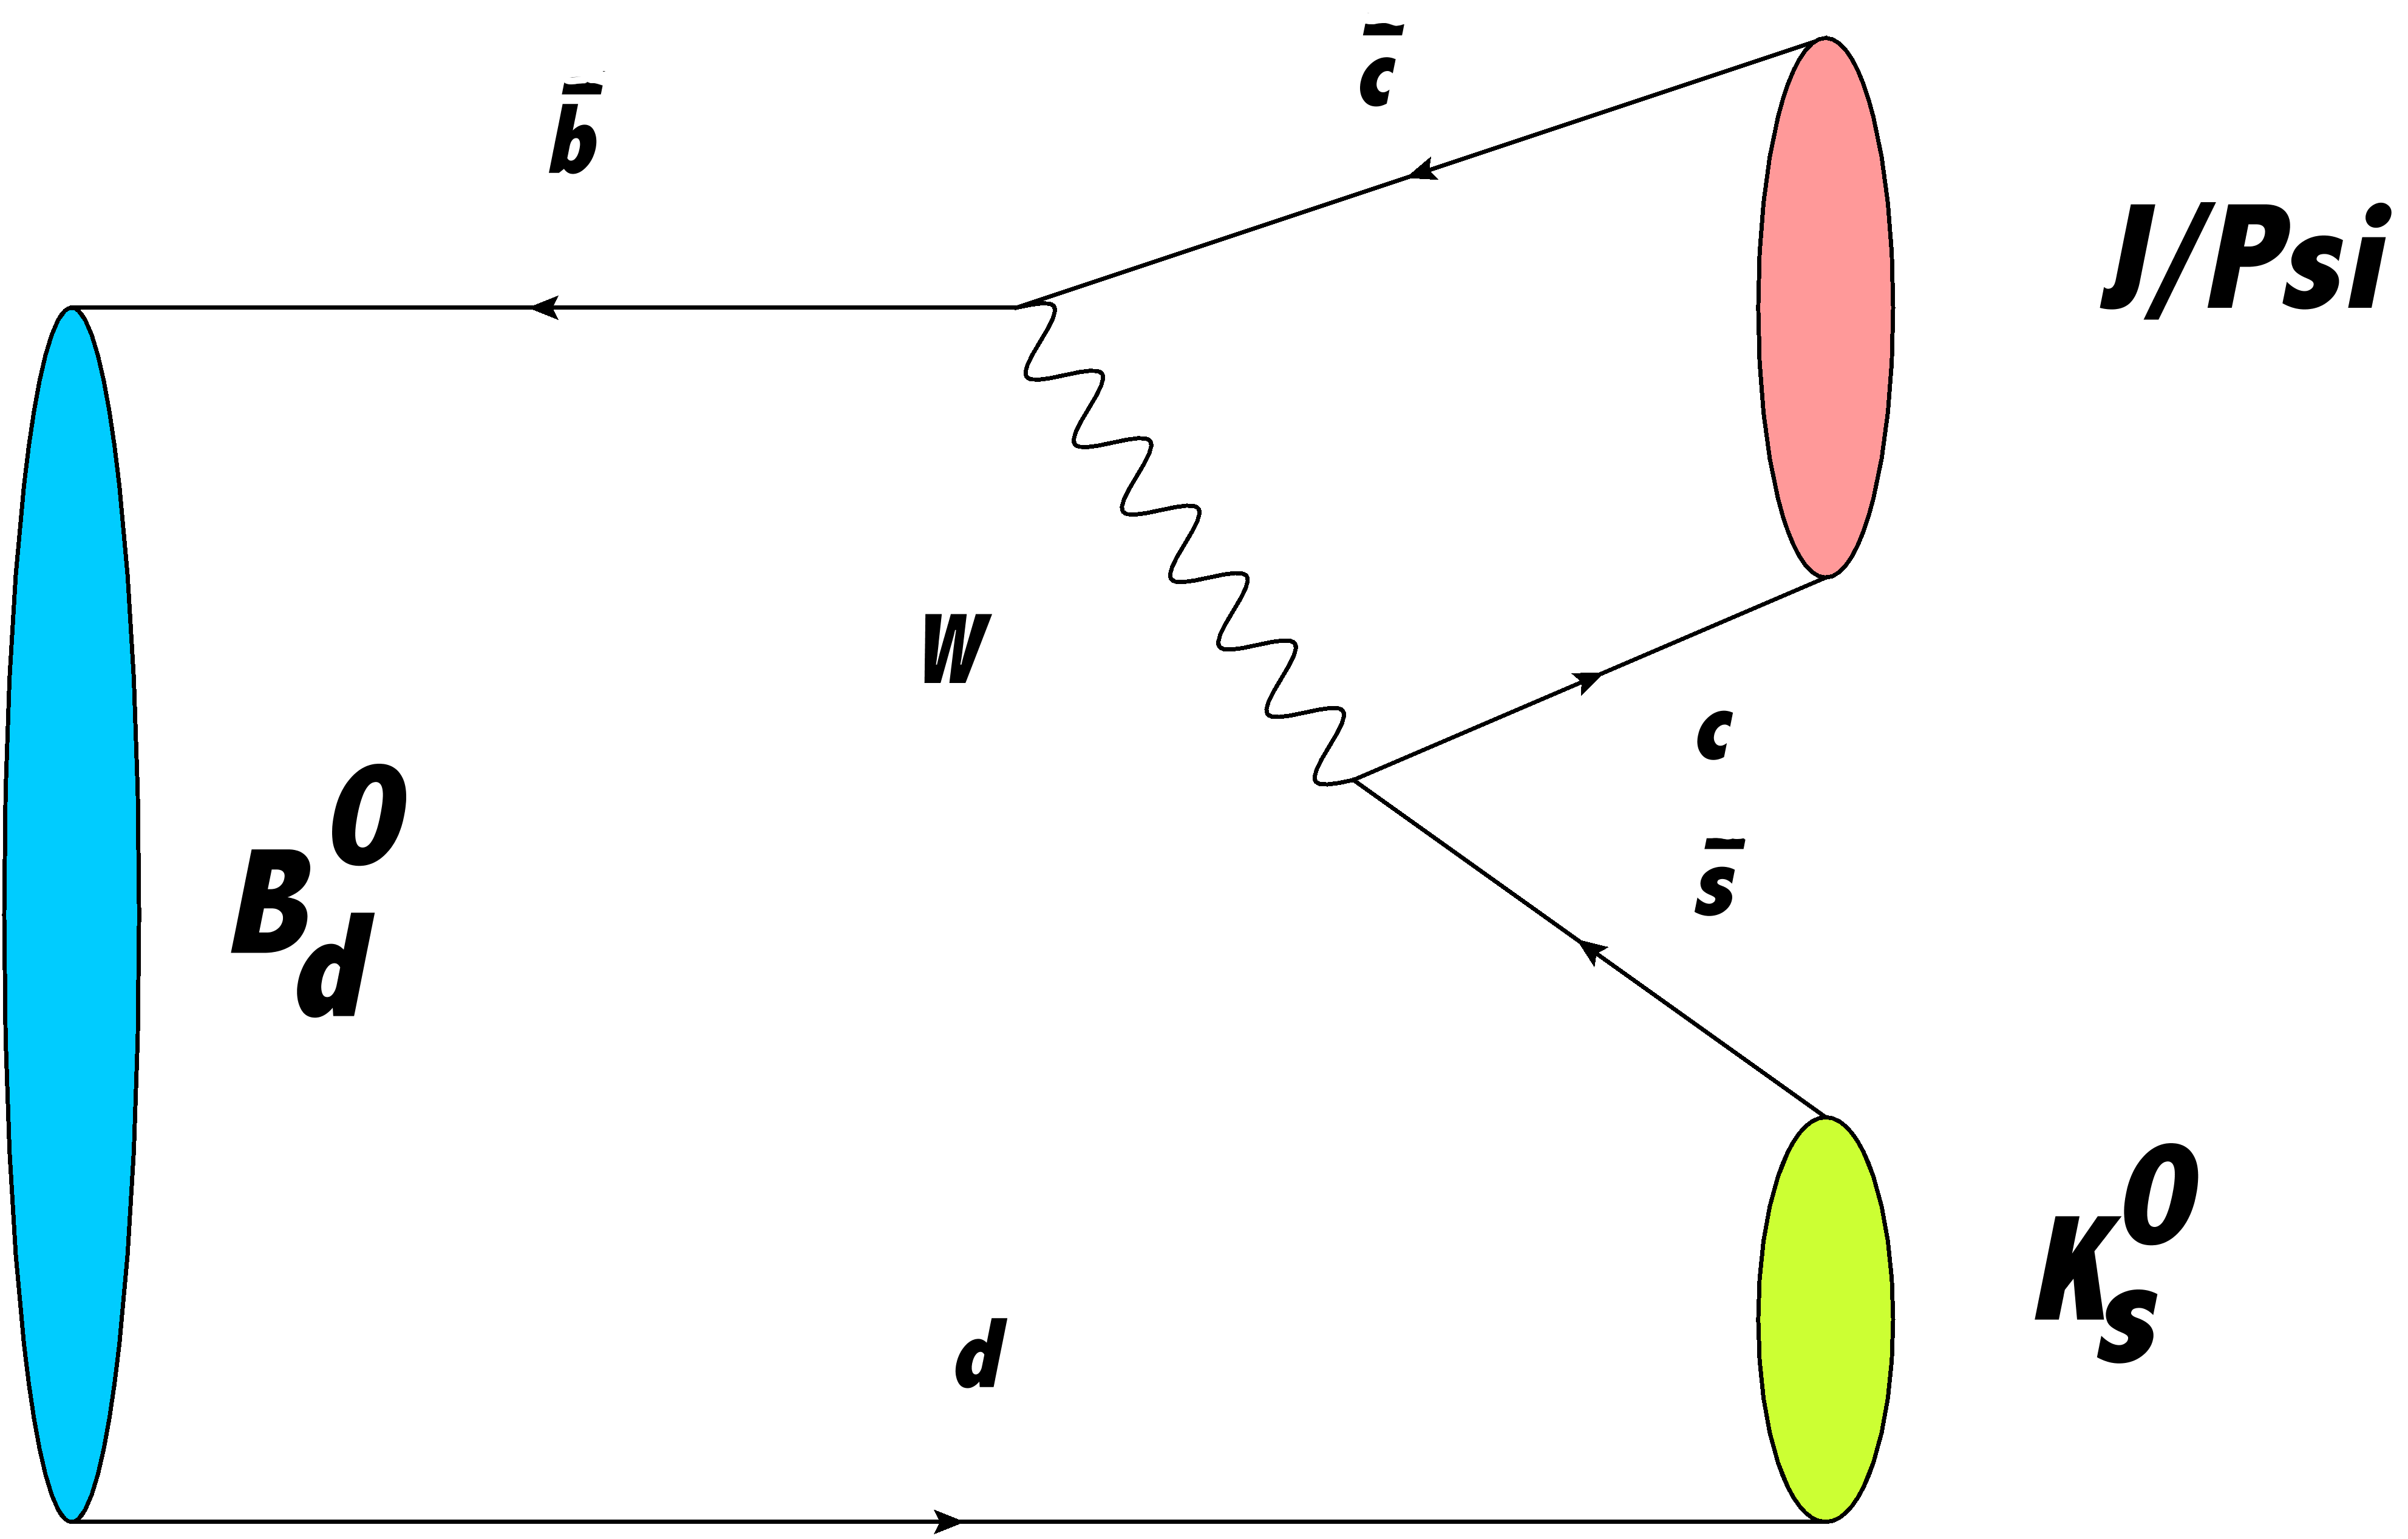
\includegraphics[width=\textwidth]{Decay}
	\end{frame}
	
	\begin{frame}{$B_d^0-\bar{B}_d^0$-Mixing}
	
\includegraphics[width=\textwidth]{Mixing}
	\end{frame}
	
	\begin{frame}{Time-dependent asymmetry}
	\begin{align}
	\mathcal{A}_{J/\Psi K_s^0}(t) &= \frac{\Gamma(\bar{B}_d^0 \rightarrow J/\Psi K_s^0)-\Gamma(B_d^0 \rightarrow J/\Psi K_s^0)}{\Gamma(\bar{B}_d^0 \rightarrow J/\Psi K_s^0)+\Gamma(B_d^0 \rightarrow J/\Psi K_s^0)} \\
		&= S_{J/\Psi K_s^0}\sin(\Delta m_d t) - C_{J/\Psi K_s^0}\cos(\Delta m_d t)
	\end{align}
	\begin{columns}
	\column{0.5\textwidth}
	\begin{block}{sine - term}
	\begin{itemize}
		\item interference between direct decay and decay after mixing
		\item $S_{J/\Psi K_s^0} = \sin(2\beta)$
	\end{itemize}
	\end{block}
	
	\column{0.5\textwidth}
	\begin{block}{cosine - term}
	\begin{itemize}
		\item interference between decay amplitudes or CPV in mixing
		\item here: $C_{J/\Psi K_s^0} \approx 0$
	\end{itemize}
	\end{block}
	\end{columns}
	\end{frame}
	
	\begin{frame}{LHCb-detector}
	\begin{center}
	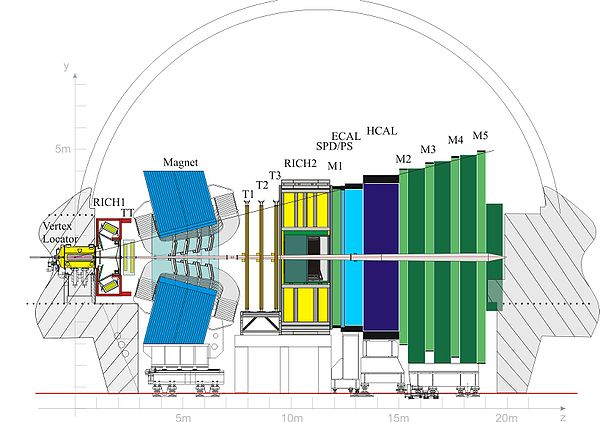
\includegraphics[width = 0.6\textwidth]{detector}
	\end{center}
	\begin{block}{Tracks}
	\begin{itemize}
		\item Long Tracks: VELO + T Stations (Johannes)
		\item Downstream Tracks: TT + T Stations (Patrick)
	\end{itemize}
	\end{block}	
	\end{frame}
	
	
	\begin{frame}{Cuts}
	\begin{center}
	\begin{tabular}{l|c|c}
	& Long Tracks & Downstream Tracks \\ \hline \hline
	candidates & 10842 & 57153 \\ \hline
	S/B & 18.0 & 4.0\\ \hline 
	cuts & & \\
	$\frac{\chi^2_{Track}}{nDof}(\mu)$ & $< 2.5$ & $< 3$ \\
	$p_T(K_s^0)$ & $> 1000$ MeV & --- \\
	$\frac{\chi^2_{Track}}{nDof}(\pi)$ & $< 1.5$ & $< 3$ \\
	$\frac{\tau}{\sigma_{\tau}}(K_s^0)$ & $> 15$ & $> 5$ \\
	decay length sig. $(K_s^0)$ & $> 25$ & $> 5$ \\
	$|M(\pi^+\pi^-)-M(K_s^0)|$ & $< 7$ MeV & $< 22$ MeV \\
	\end{tabular}	
	\end{center}
	New in 2012: Ghost probability. We choose ghost prob $<0.5$.
	\end{frame}
	
	\begin{frame}{Fit strategy}
	\begin{itemize}
	\item Unbinned Maximum Likelihood Fit
	\item sFit: Maximise modified likelihood function
	\begin{align}
	test
	\end{align}
	\item sWeigths calculated with sPlot-technique
	\end{itemize}
	\begin{align}
	\mathcal{P}_{meas} = \underbrace{\epsilon(t)}_{= 1, \text{later more}}\mathcal{P}_{sig}(t') \otimes \mathcal{R}(t-t')
	\end{align}
	\end{frame}
	
	\begin{frame}{Mean dacay time resolution}
	Resolution model
	\begin{align}
	\mathcal{R}(t) = \sum_{i=0}^3 \frac{f_i}{2\pi\sigma_i}e^{-\tfrac{t^2}{2\sigma^2}}
	\end{align}
	Perform sFit with reonstructed $J/\Psi$ mass as discriminating variable
	\end{frame}
	\begin{frame}{Mean dacay time resolution}
		\begin{columns}
	\column{0.5\textwidth}
	\begin{block}{Long Tracks}
	%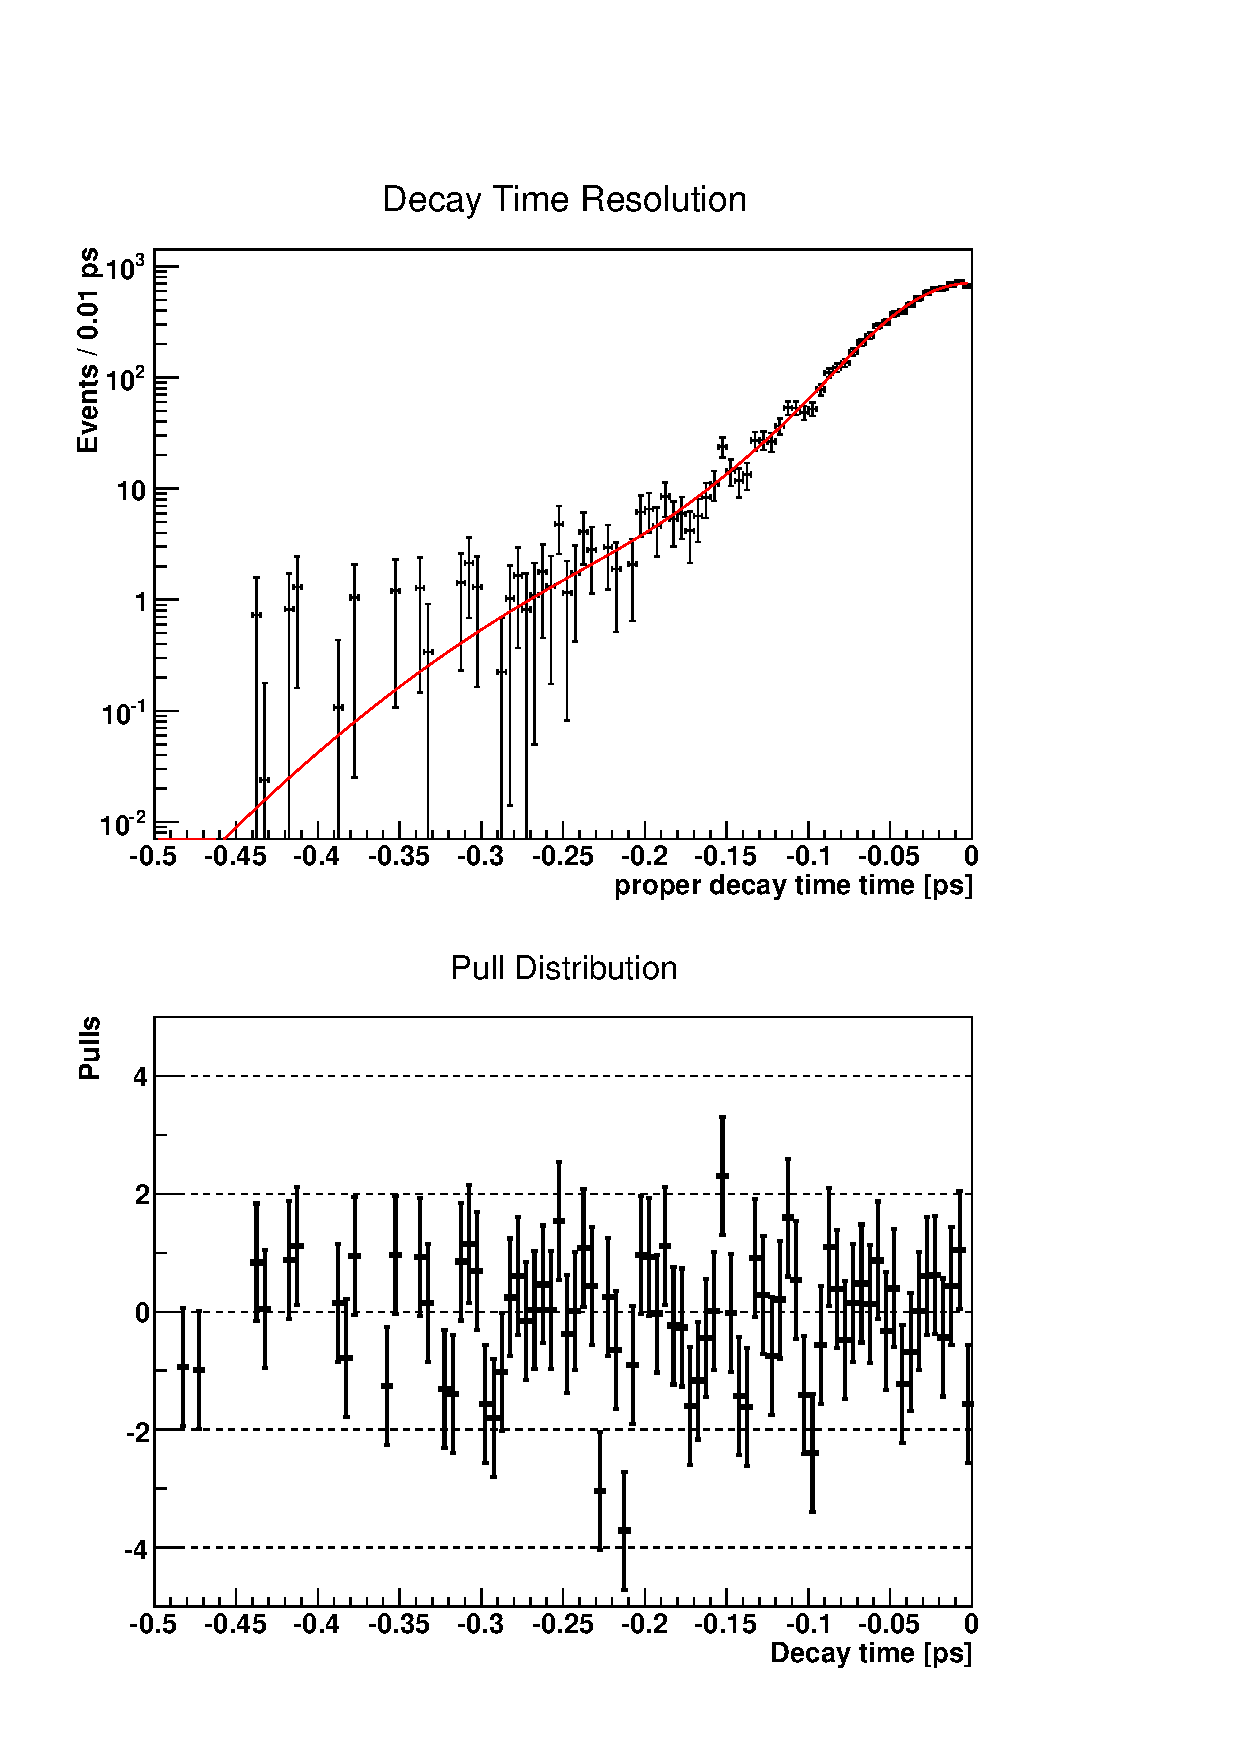
\includegraphics[width=\textwidth]{resolution_lt}
	\end{block}
	\column{0.5\textwidth}
	\begin{block}{Downstream Tracks}
	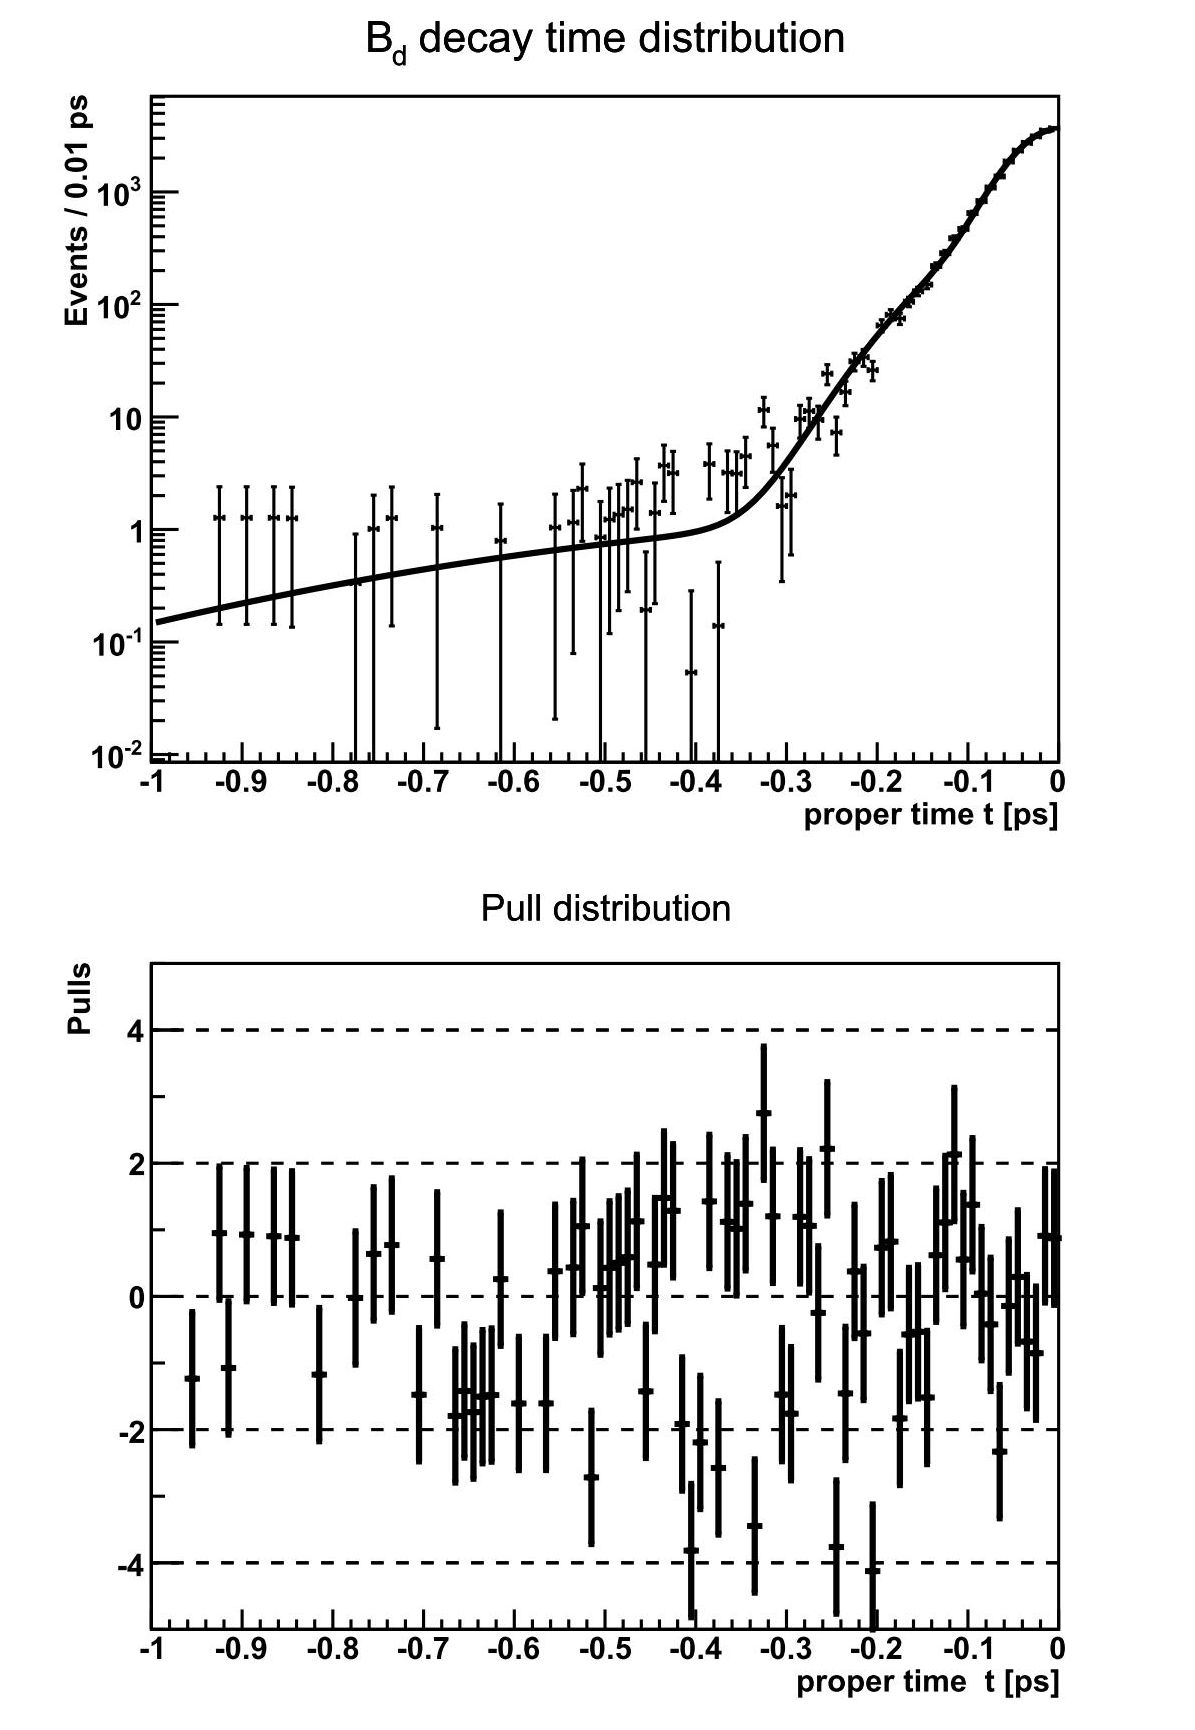
\includegraphics[width=\textwidth]{resolution_ds}
	\end{block}
	\end{columns}
	\end{frame}

    \begin{frame}{Resolution}
    \begin{center}
    $\begin{array}{l | r@{\pm}l | r@{\pm}l}
\hline 
\hline
\text{Parameter} & \multicolumn{2}{c|}{\text{long tracks}} & \multicolumn{2}{c}{\text{downstream tracks}}\\
\hline
\sigma_{1}\hspace{1cm}(\text{ps}) &	0.117 & 0.016 & 0.480 & 0.070\\
\sigma_{2}\hspace{1cm}(\text{ps}) &	0.061 & 0.037 & 0.04396 & 0.00094\\
\sigma_{3}\hspace{1cm}(\text{ps}) &0.037 &	0.003 & 0.0932 & 0.0034 \\
f_{1} &0.054 & 0.032 & 0.00329 & 0.00099\\
f_{2} &0.294 & 0.138 & 0.739 & 0.027\\ \hline \hline
\end{array}$   
    \end{center}
    \end{frame}        	
	
	\begin{frame}{nominal fit}{mass fit - parameterisation}
	\begin{block}{Signal}
	\begin{align}
\mathcal{P}_{m;S}(m;\vec{\lambda}_{m;S}) = f_{S,m}\mathcal{G}(m;m_{\text{\Bd}},\sigma_{m,1}) + \mathcal{G}(m;m_{\text{\Bd}},\sigma_{m,2})
\end{align}
\end{block}
\begin{block}{Background}
\begin{align}
\mathcal{P}_{m;B}(m;\vec{\lambda}_{m;B}) = \frac{1}{\mathcal{N}_{m;B}}e^{-\alpha_m m}
\end{align}
\end{block}
\begin{block}{Total mass p.d.f.}
\begin{align}
\mathcal{P}_{m}(m;\vec{\lambda}_{m}) = f_{sig}\mathcal{P}_{m;S}(m;\vec{\lambda}_{m;S}) + (1-f_{sig})\mathcal{P}_{m;B}(m;\vec{\lambda}_{m;B})
\end{align}
\end{block}
	\end{frame}
	
	\begin{frame}{nominal fit}{mass fit}
	\begin{columns}
	\column{0.5\textwidth}
	\begin{block}{Long Tracks}
	%\includegraphics[width=\textwidth]{fit_mass_lt}
	\end{block}
	\column{0.5\textwidth}
	\begin{block}{Downstream Tracks}
	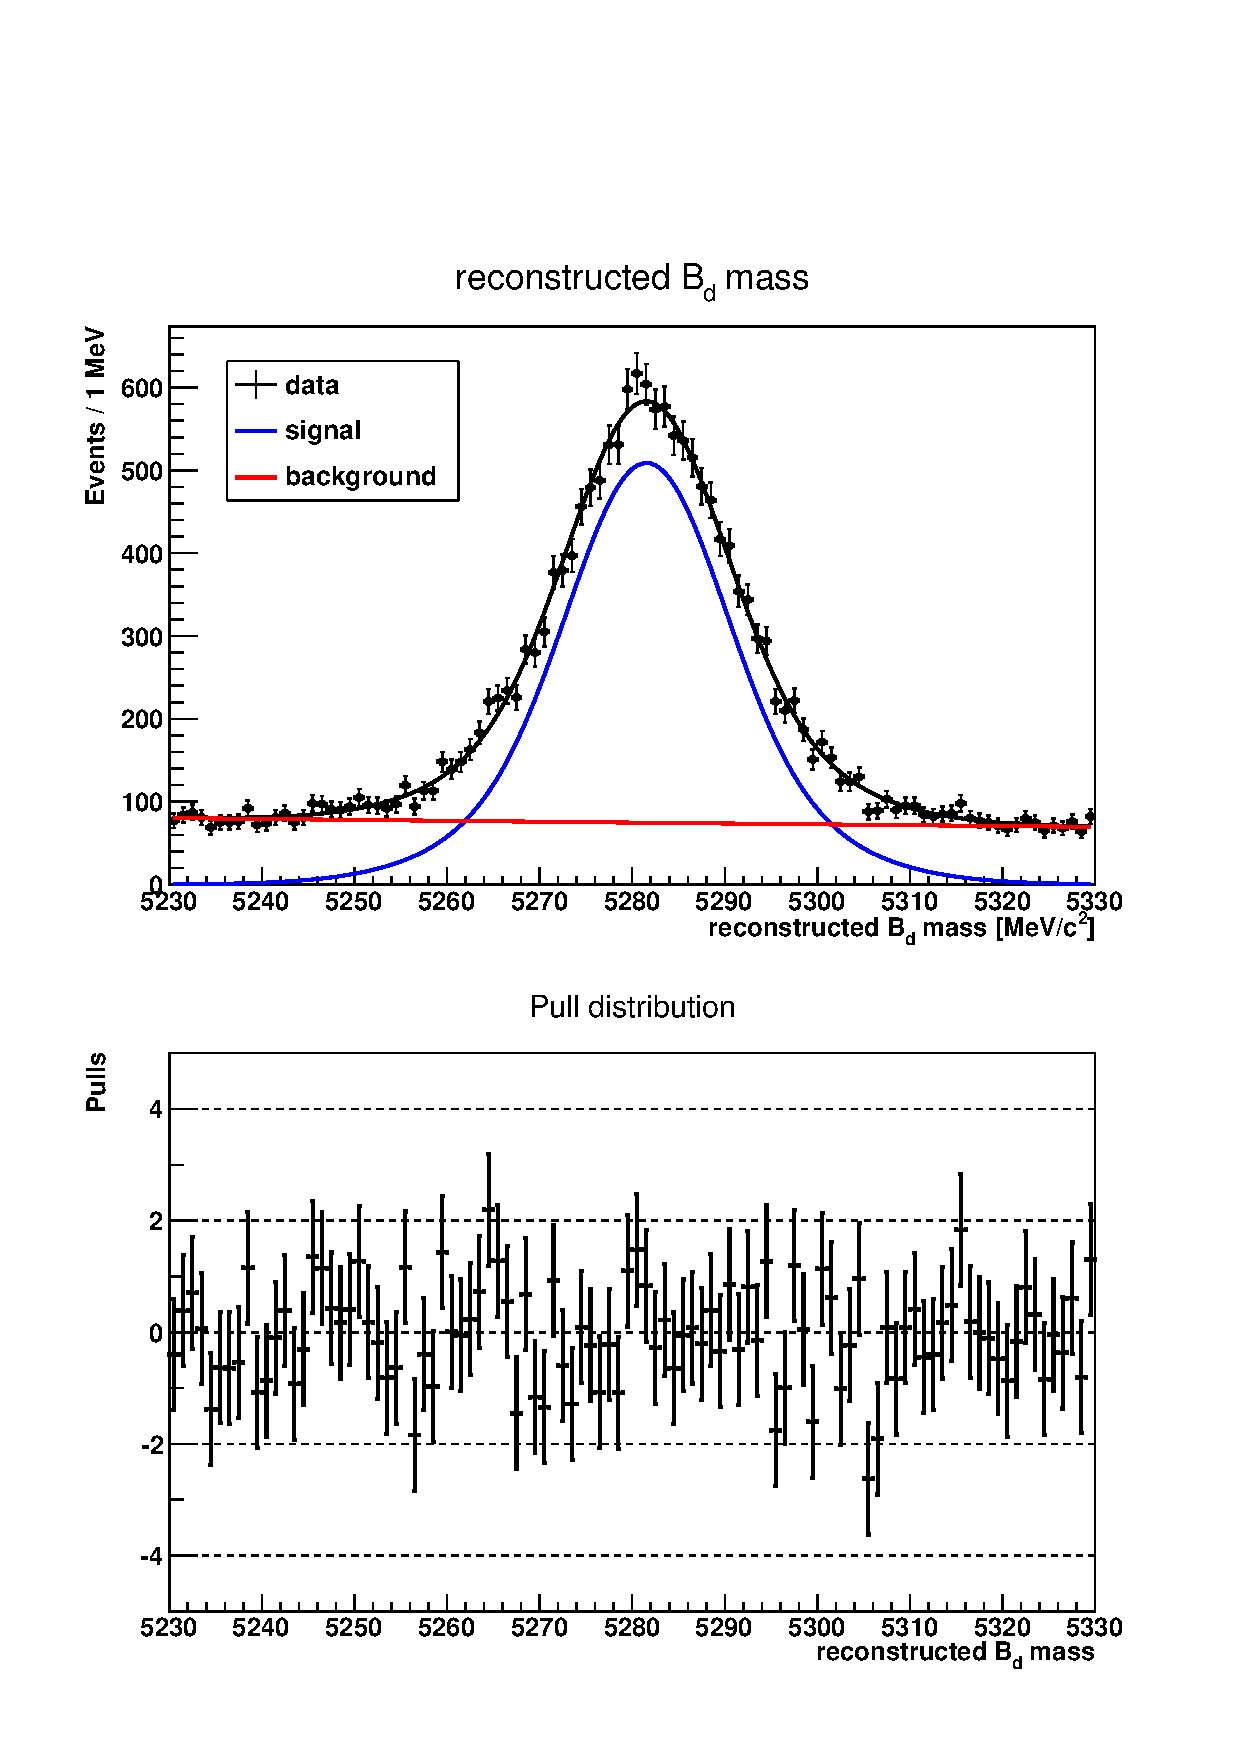
\includegraphics[width=\textwidth]{mass_fit_ds}
	\end{block}
	\end{columns}
	\end{frame}
	
	\begin{frame}{nominal fit}{Probability density function}
	\begin{align}
\nonumber\mathcal{P}_{\text{meas}}(t, d, \omega) \propto &e^{-t/\tau} \left\lbrace 1-d\mu(1-2\omega)-d\Delta p_0 \right. \\
&- \left.\left[d(1-2\omega)-\mu(1-d\Delta p_0)\right]\SJPsi\sin(\Delta m_d t)\right\rbrace
	\end{align}
	
	\begin{itemize}
		\item d: tagging decision
		\item $\mu = A_P = \frac{R_{\bar{B}_d^0}-R_{B_d^0}}{R_{\bar{B}_d^0}+R_{B_d^0}}$ production asymmetry
		\item $\omega$: calibrated mistag probability
		      \begin{align}
		      (\eta^{OS}) = p_1 (\eta^{OS} - \left\langle \eta^{OS} \right\rangle) + p_0
		      \end{align}
		      $p_0, p_1$: calibration parameters \\
		      $\eta^{OS}$: predicted mistag probability
		\item $\Delta p_0$: tagging calibration asymmetry
		\item $\Delta m_d$: mixing frequency

	\end{itemize}	
	\end{frame}
	
	
	
	\begin{frame}{Fit results}
	\begin{itemize}
		\item floating parameters: $S_{J/\Psi K_s^0}$, $\tau$, $\Delta m_d$
		\item constrained parameters: $\mu = -0.015\pm0.013$, $p_0 = 0.382\pm0.003$, $p_1=0.981\pm0.024$, $\Delta p_0 = 0.0045\pm0.0053$
		\item fixed parameters: $\left\langle \eta^{OS} \right\rangle = 0.382$, resolution parameters
		\item signal events: ??? (long) // 8585 (downstream) [2011: 8600 total]
	\end{itemize}
	\end{frame}

	
	\begin{frame}{Fit results}
	\begin{columns}
	\column{0.5\textwidth}
	\begin{block}{Long Tracks}
	%\includegraphics[width=\textwidth]{decay_lt}
	\end{block}
	\column{0.5\textwidth}
	\begin{block}{Downstream Tracks}
	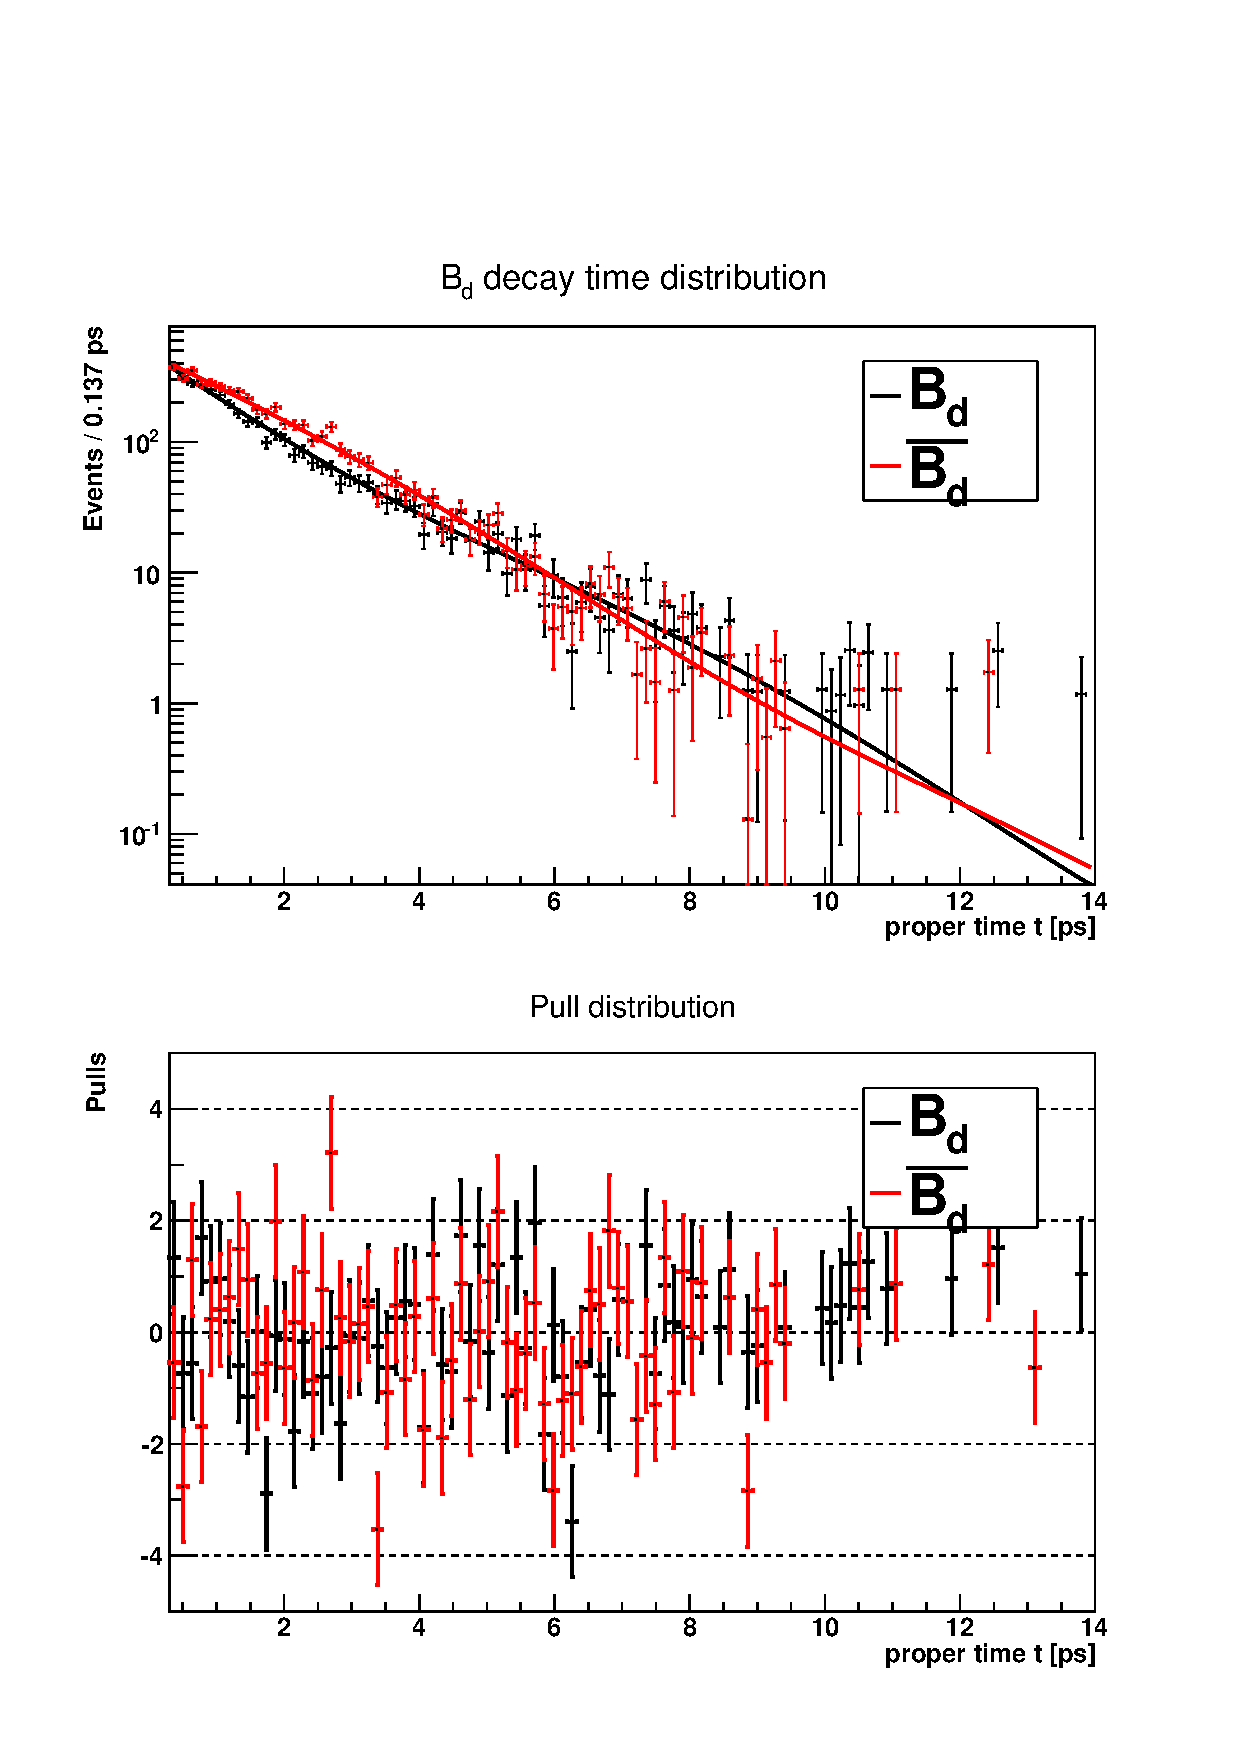
\includegraphics[width=\textwidth]{decay_distribution_ds}
	\end{block}
	\end{columns}

	\end{frame}
	
	\begin{frame}{fit results}
	\begin{center}
	$\begin{array}{l r@{\pm}l r@{\pm}l}
	\hline \hline
	Parameter & \multicolumn{2}{c}{\text{long}} & \multicolumn{2}{c}{\text{downstream}} \\ \hline
	\SJPsi     & & & 0.565 & 0.069 \\
	\tau       & & & 1.516 & 0.039 \\
	\Delta m_d & & & 0.521 & 0.039 \\
	\hline
	\end{array}$
	\end{center}
	\end{frame}

	
	\begin{frame}{Systematic errors}
	\begin{itemize}
		\item Fit Bias due to fit method
	    \item Tagging calibration
	    \item Time acceptance
	    \item Correlation mass $\leftrightarrow$ decay time
	    \item Time resolution
	\end{itemize}
	\end{frame}
	
	\begin{frame}{Systematic Errors}{Fit Bias}
	Generate Toy MC with ??? (long) / 13000 events an parameters derived from nominal fit (except $\SJPsi = 0.75$)
	\begin{columns}
	\column{0.5\textwidth}
	\begin{block}{Long Tracks}
	%\includegraphics[width=\textwidth]{pulls_s_lt}
	\end{block}
	\column{0.5\textwidth}
	\begin{block}{Downstream Tracks}
	%\includegraphics[width=\textwidth]{pulls_s_ds}
	\end{block}
	\end{columns}
	\end{frame}
	
	\begin{frame}{Systematic errors}{Tagging calibration}
	Vary Tagging calibration parameters $p_0, p_1$ $\pm$ their systematic uncertainties
	\begin{enumerate}
	\item in the nominal fit
	\item in the generation of Toy MC, but fit with original values
	\end{enumerate}
	\begin{alert}{Note:}
	Systematic studies on used tagging calibration hasn't finished yet $\longrightarrow$ no official value. We use largest differences in channels so far:
	\begin{align*}
	\delta p_0^{stat.} = 0.019, \qquad \delta p_1^{stat.} = 0.07
	\end{align*}
	\end{alert}
	\end{frame}
	
	\begin{frame}{Systematic errors}{Tagging calibration}
	Choose highest difference from nominal fit / toy as estimate for the systematic uncertainty
	\begin{itemize}
	\item Long tracks:
	\item Downstream tracks:
    \end{itemize}		    
    \begin{alert}{Note:}
    Estimates very large due to large $\delta p_0^{stat.}$, $\delta p_1^{stat.}$ compared to other calibrations (systematic studies of calibration need to be finished)
    \end{alert}
    \end{frame}
    
    \begin{frame}{Systematic errors}{Time acceptance}
    \begin{alert}{Note:}
    just a cross-check, no in-depth analysis
    \end{alert}
    \begin{block}{Determination of an acceptance function}
    \begin{itemize}
    \item no separation between \Bd and \Bdbar \\
          $\Rightarrow$ simple exponential decay
    \item neglect lifetime cut ($t > 0.3\text{ps}$)
    \item contributions to acceptance:
          \begin{itemize}
          \item turn-on-effect
          \item decreasing acceptance for higher lifetimes due to VELO geometry
          \end{itemize}
    \end{itemize}
    \end{block}
\end{frame}

\begin{frame}{Systematic errors}{Time acceptance}
    \begin{block}{Fit p.d.f}
    $\mathcal{P}_{acc}(t) \propto \underbrace{e^{-t/\tau}}_{\text{exp. decay}} \cdot \underbrace{\frac{2}{\pi}\arctan[t\cdot \exp(at+b)]}_{\text{turn-on-effect}} \cdot \underbrace{(1 + \beta t)}_{\substack{\text{higher lifetimes} \\(\beta<0)}}$
    \end{block}
    \begin{alert}{Note:}
    $\tau$ will be constrained to the PDG value $\tau = 1,519 \pm 0,007 \pico\second$.
    \end{alert}
\end{frame}

\begin{frame}{Systematic errors}{Time acceptance}
\begin{block}{Long Tracks}
%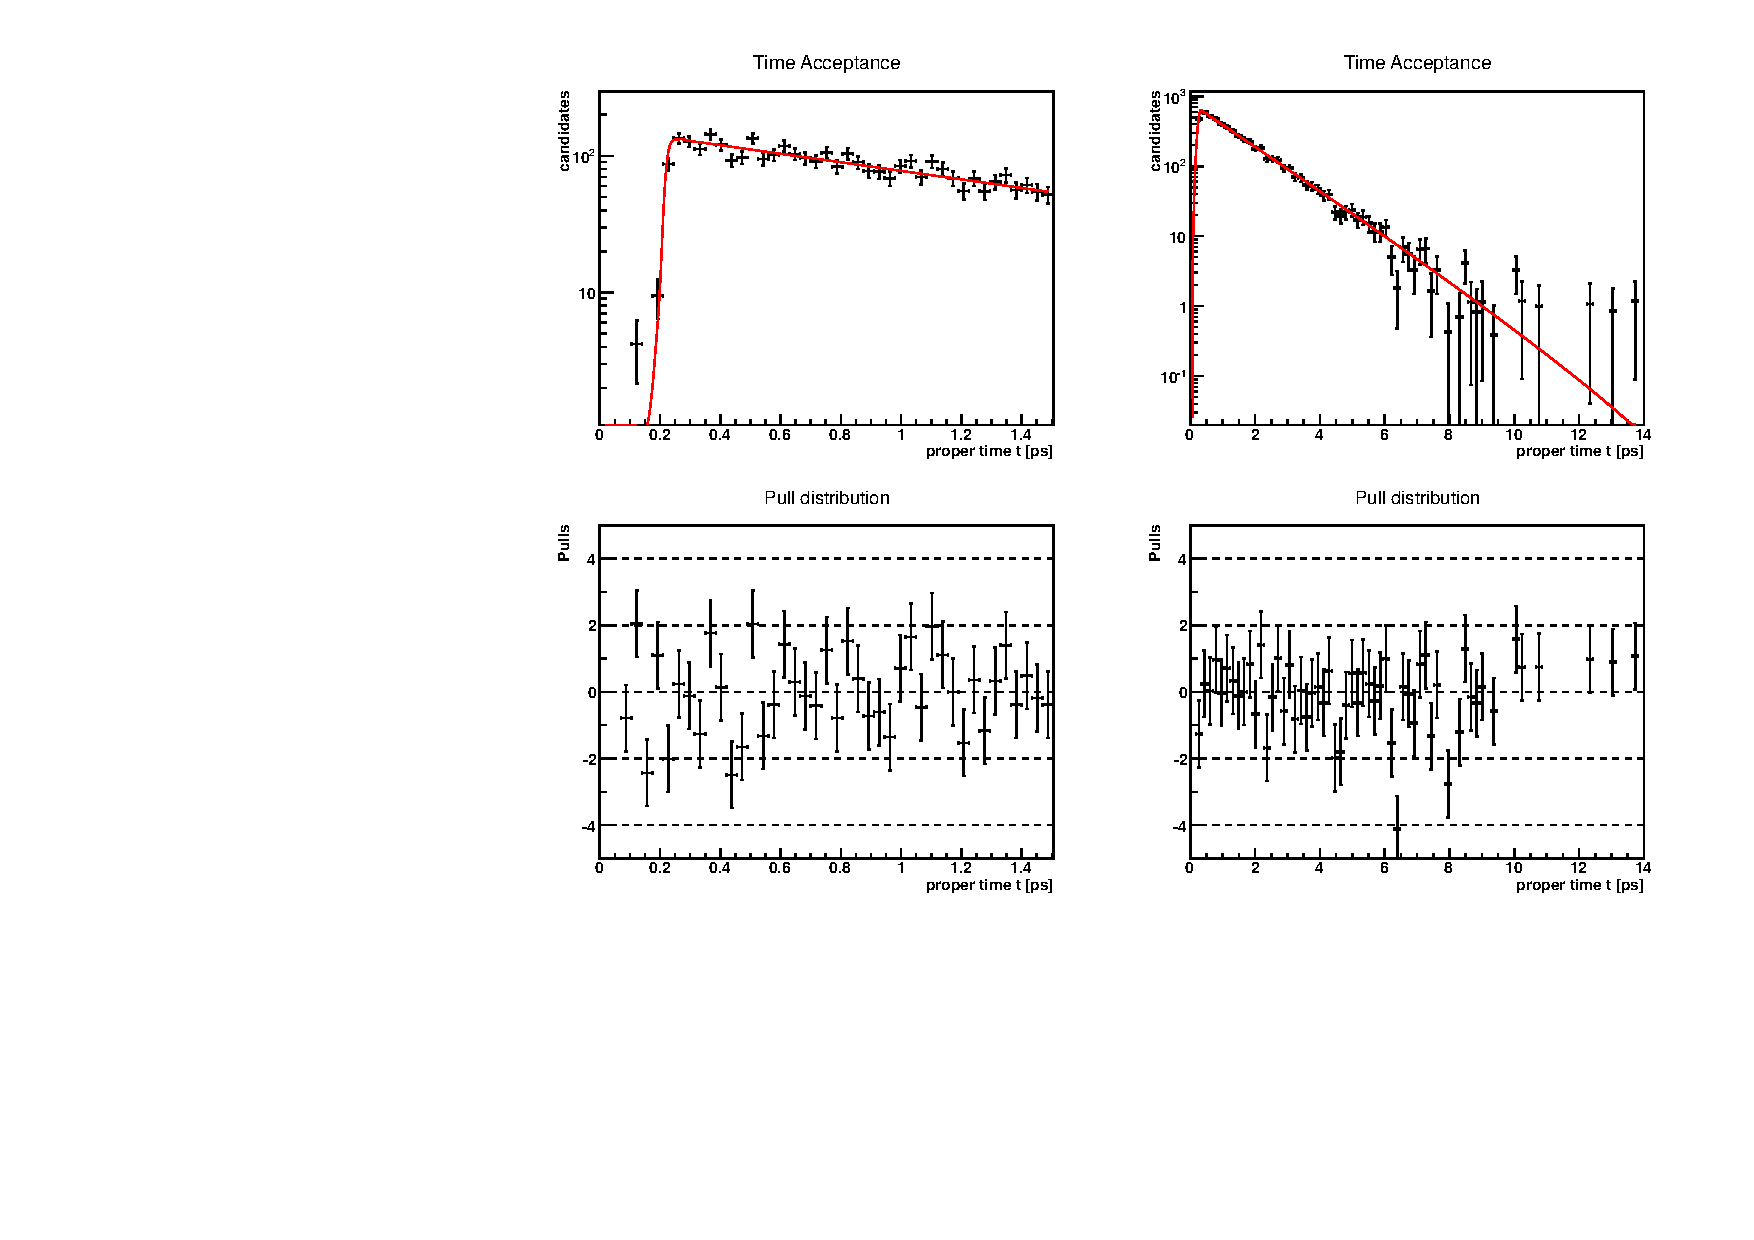
\includegraphics[width=\textwidth]{time_acceptance_fit_lt}
\end{block}
\end{frame}

\begin{frame}{Systematic errors}{Time acceptance}
\begin{block}{Downstream Tracks}
%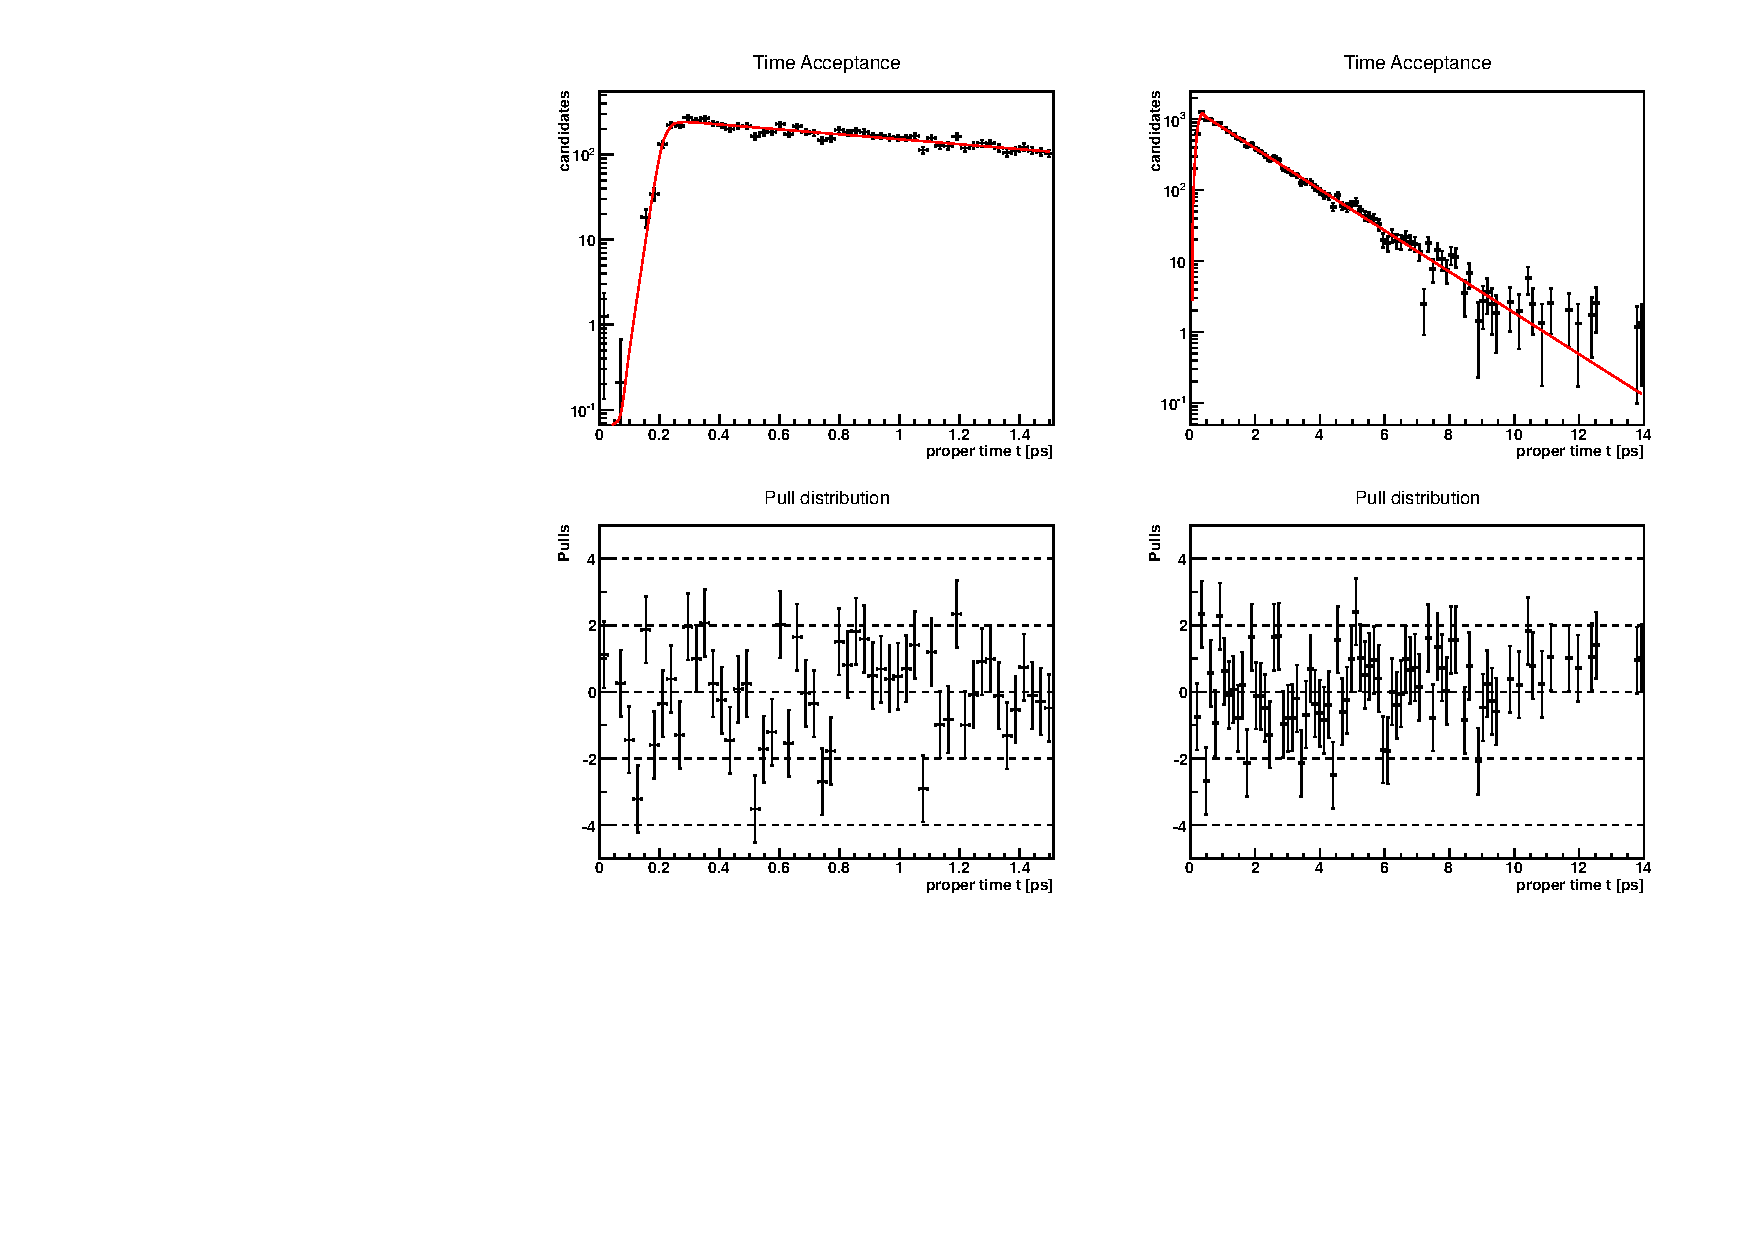
\includegraphics[width=\textwidth]{time_acceptance_fit_ds}
\end{block}
\end{frame}

\begin{frame}{Systematic errors}{Time acceptance}
\begin{table}
\caption{Fit results for exponential decay fit with acceptance function. $\tau$ was constrained to the PDG value $\tau = 1,519 \pm 0,007 \pico\second$}
\begin{tabular}{lr@{$\pm$}l r@{$\pm$}l}
\hline \hline 
parameter & \multicolumn{2}{c}{long} & \multicolumn{2}{c}{long} \\ \hline
$\tau$    & & &  1.519   & 0.007 \\
$a$       & & &  44.1    & 5.7 \\
$b$       & & &  -7.4    & 1.1 \\
$\beta$   & & &  -0.0056 & 0.0085 \\ 
\hline \hline
\end{tabular}
\end{table}
\end{frame}

\begin{frame}{Systematic errors}{Time acceptance}
Toy MC Study
\begin{itemize}
\item generate with acceptance function 
\item use parameters mentioned above
\item fit without acceptance function
\end{itemize}
%\includegraphics[width=\textwidth]{time_acceptance_toys}
\begin{center}
No significant difference to fit bias! \\
$\mu_{fit} = 0.059 \pm 0.007 \quad \text{vs.} \quad \mu_{acc} = 0.063 \pm 0.007$
\end{center}
\end{frame}

\begin{frame}{Systematic errors}{Correlation mass $\leftrightarrow$ decay time}

\end{frame}

\begin{frame}{Systematic errors}{Resolution}

\end{frame}

\begin{frame}{Systematic errors}{Summary}
\begin{center}
\begin{tabular}{l c c}
\hline \hline
effect & long & downstream \\ \hline
fit  method & & \\
tagging calibration & & \\
time acceptance & & \\
mass $\leftrightarrow$ decay time & & \\
resolution & & \\ \hline
total & & \\
\hline \hline
\end{tabular}
\end{center}

\end{frame}

\begin{frame}{Conclusion}

\end{frame}

% Backup-Folien
% =============
% - Trigger-Definitionen
% - sFit erklären

\end{document}